%Overview of existing technology (hardware)

\chapter{Overview of Existing Technology}
\section{PLC Hardware Controller Implementations}
%link to automotive statement: http://www.amci.com/tutorials/tutorials-what-is-programmable-logic-controller.asp
Programmable Logic Controllers (PLC) have been around for over 30 years and as such there have been many iterations and designs. The original Programmable Logic Controllers came into being to fill the need of automotive manufacturers replacing traditional relays with digital control. These relays were hooked up to power rails and inputs and allowed for basic mechanical logic to be performed. Due to their mechanical nature relays wore out over time causing the logic programmed using them to fail. In addition because hundreds to thousands could be used in a cabinet were also difficult to isolate the worn out part. Relays also proved to be inflexible when a small change was required to be added to the program, the entire plant was required to be taken offline in order to make the change. Halting large production plants is often extremely costly and thus eventually the relays were migrated out in favor of microcontrollers that can be reprogrammed on the fly. To this day modern PLC's still use graphical analogies of circuits and relays in order to construct their programmable logic. This visual language is now referred to as ladder logic due to the the finished program having a similar structure to a conventional ladder. 

\begin{figure}[htp]
    \centering
    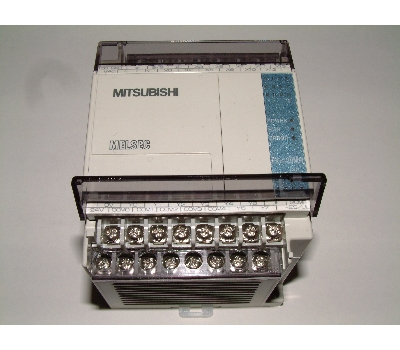
\includegraphics[width=\imgmedphoto]{./images/c01_mitsubishiplc.jpg}
    \caption{Mitsubishi PLC All In One Unit \cite{img_c01_MitsubishiPlc}}
    \label{img:mitsubishiplc}
\end{figure}

Mitsubishi Automation\ref{img:mitsubishiplc}, Siemens, and Omron are just a few of the big producers of industry standard PLC's although the shape and form factor differ between manufacturers differ PLC's always consist of 3 distinct parts.  The input module, the main controller unit and the output module (please refer to figure \ref{plcrender_1}). This separation exists due to varying requirements for analog inputs and different output level requirements in order to drive heavy machinery. I/O modules may consist of thermo sensors, ambient light sensors, resistive sensors, or a direct connection the the external circuitry. Likewise the output module may also be composed of both analog or digital output pins.

\begin{figure}[htp]
    \centering
    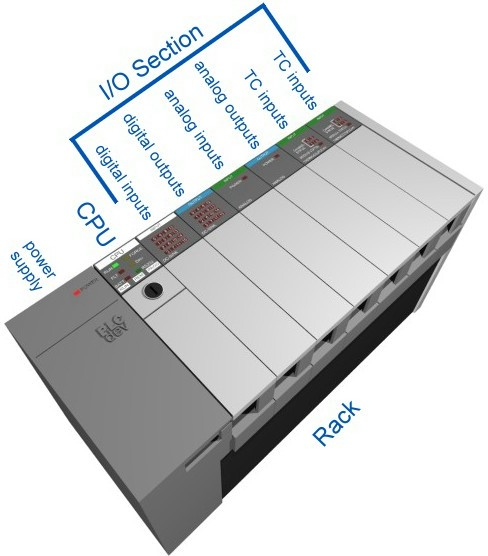
\includegraphics[width=\imgmedphoto]{./images/c02_plcdev.jpg}
    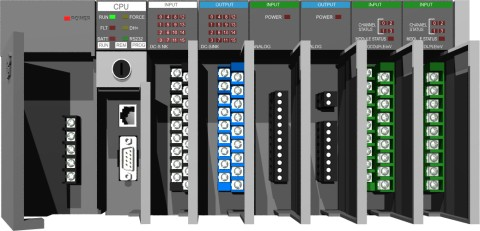
\includegraphics[width=\imgmedphoto]{./images/c04_plcdev.jpg}
    \caption{3D Diagram of A Modular PLC \cite{img_c02_PlcDev,img_c04_PlcDev}}
    \label{img:plcrender_1}
\end{figure}

%source http://www.sea.siemens.com/step/templates/lesson.mason?plcs:2:3:1
Programs are executed from the main PLC control unit. An iteration of execution is refered to as a scan. A scan is broken up into 4 phases: Self-Test, Input scan, Logic solve / scan, and Output scan. Figure \ref{fig:plcexecution} shows the order in which these steps are executed. Each step contains various jobs, in more detail they are:

\pagebreak{4}

\begin{figure}[htp]
    \centering
    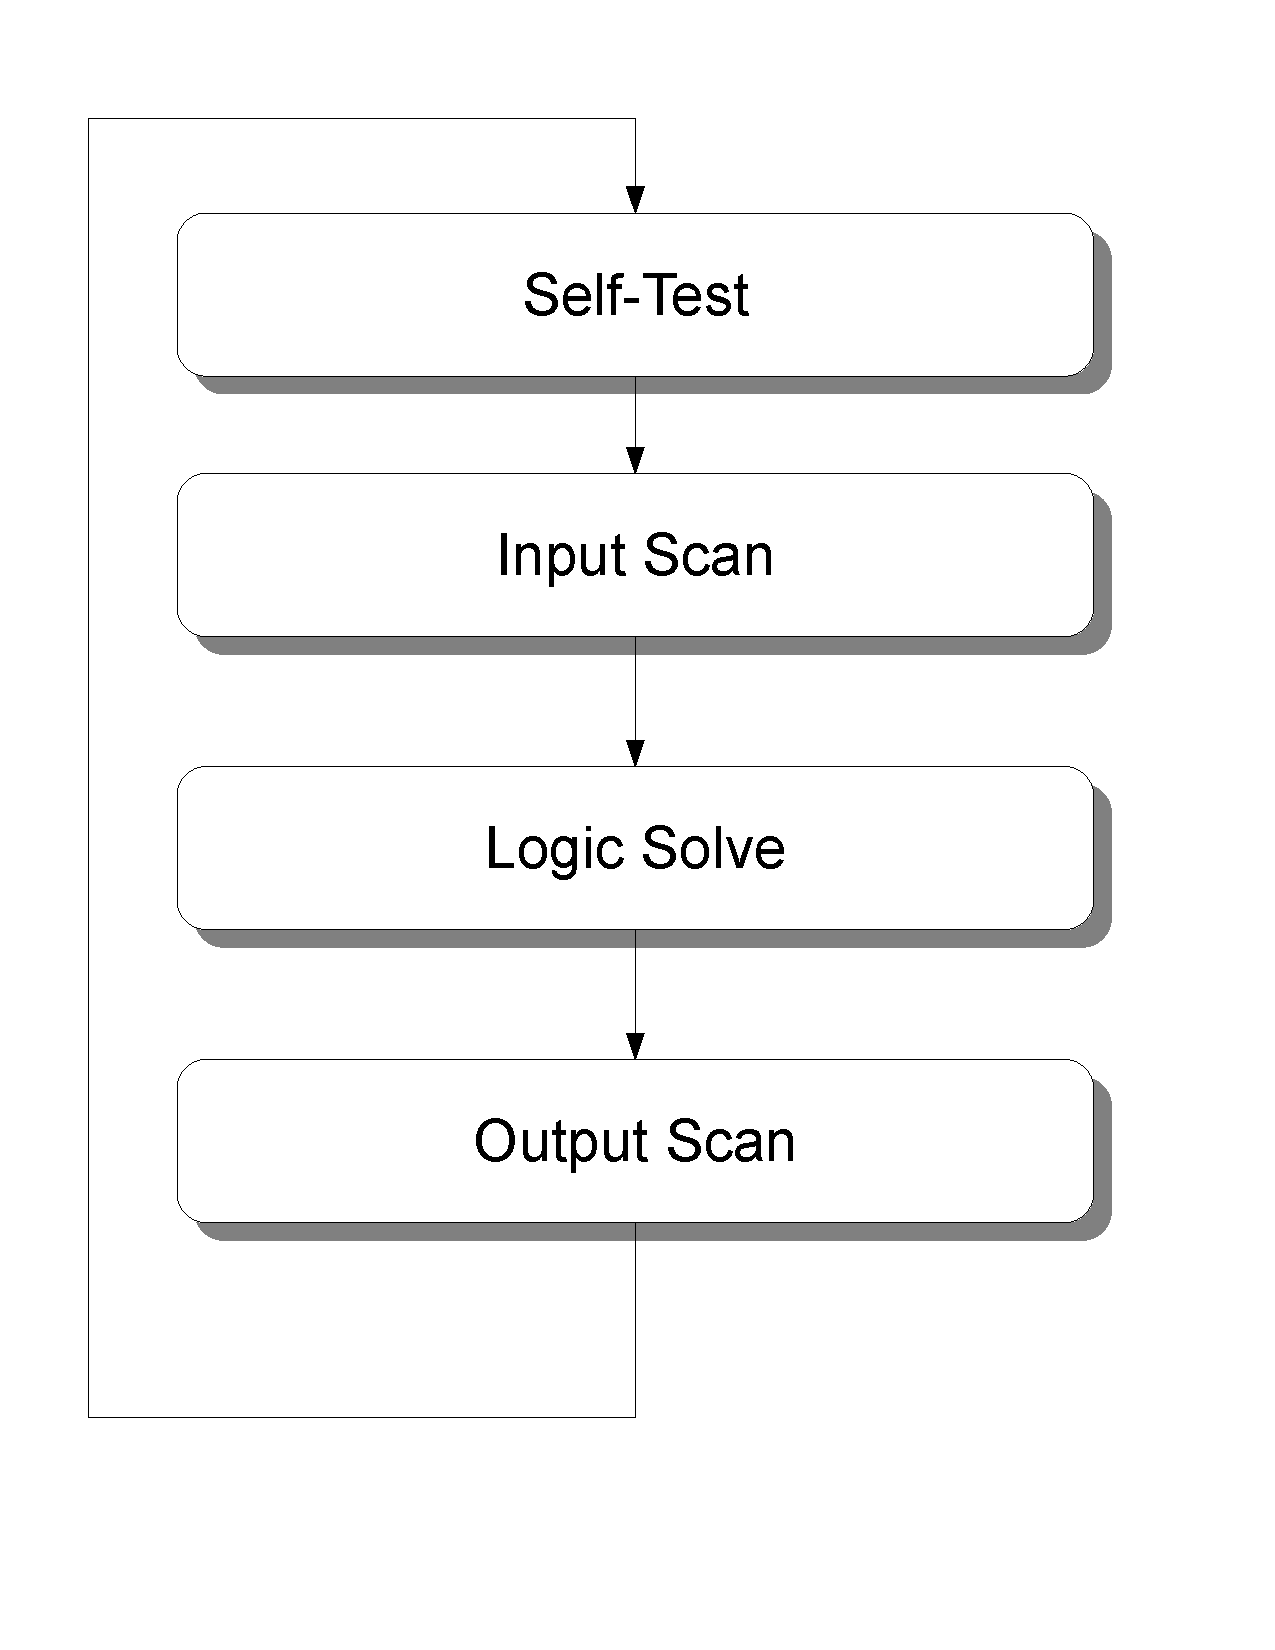
\includegraphics[width=\imgmedphoto]{./images/plcexecution.pdf}
    \caption{PLC Execution Loop}
    \label{fig:plcexecution}
\end{figure}

%todo: draw a flow chart of the following stages
\begin{itemize}
	\item\textbf{Self-Test:} All PLC's contain self diagnostic routines, this includes communication checks between the main control unit and the I/O modules. If a fault is found it is handled here before any of the execution is allowed to proceed.
	\item\textbf{Input Scan:} All inputs both from the input modules and from the internal memory are scaned. This is done in a single step to make sure that all future calculations for the currently executing scan has consistent data. You may note that updates are not read until the next input scan.
	\item\textbf{Logic Solve / Scan:} Calculations and computations from the user programs are computed in this step if values are to be stored back into internal registers they are now put into temporary registers. Similarily if external output is required it is written to a temporary internal register that will hold the output until the output phase is executed.
	\item\textbf{Output Scan:} Internal temporary registers are written to their destination registers in one step. External outputs take on the values held by the registers that stored data for the output modules all outputs also take place in one step.
\end{itemize}

Each of these phases semantically can be assumed to execute cocurrently thus, the order of individual instructions in each phase is of no consequence. This closely follows the Ladder Logic (please see section \ref{section:ladderlogic}) in that the entire program executes cocurrently on multiple rungs. Internally however PLC's do have a sequential deterministic order in which instructions are executed, this is a side effect of using microcontrollers in the main control unit. In this way it can be said that each phase is considered concurrent if we consider a cycle time greater than the time it takes to execute the last instruction. If an external device takes samples at this rate it is irrelevent from its perspective that the processing is not actually happening cocurrently to the observing device the two behaviors are equivalent.

\begin{figure}[htp]
    \centering
    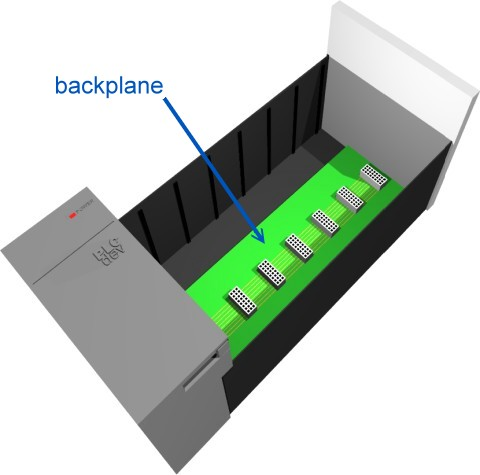
\includegraphics[width=\imgmedphoto]{./images/c03_plcdev.jpg}
    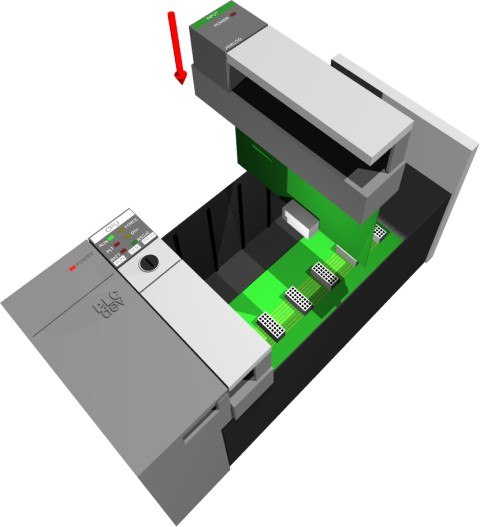
\includegraphics[width=\imgmedphoto]{./images/c05_plcdev.jpg}
    \caption{3D Diagram of A Modular PLC With One Module Being Inserted \cite{img_c03_PlcDev,img_c05_PlcDev}}
    \label{img:plcrender_2}
\end{figure}

The input and output modules generally connect to the main module via serial links however some companies also include network commuication over standard shielded ethernet\cite{rockwell_io,rockwell_tech_pub}. Generally serial communication is used more often when the input and output modules are at a close distance to the controller unit (see figure \ref{img:plcrender_2}) such as in a modular PLC design. The network interface on the other hand is used when the input or output module needs to be located far away from the main controller unit\cite{rockwell_tech_pub} as is often the case in automated production facilities. Output modules are generally relay driven and the driving current is provided by a transistor connected to logic pins of the main controller. This is done to isolate the internal circuitry from the demands of driving heavy machinery \cite{plcapp}. Alternatively some circuits employ an opto-isolator circuitry to achieve the same effect the trade off being less current under load but faster switching and better service life \cite{plcapp}. Analog outputs are obtained by passing a binary value through a DAC with some reference voltage the output voltage.

%\begin{equation}
%V_{out} = V_{ref} ( b_7/2 + b_6/4 + b_5/8 + b_4/16 + b_3/32 + b_2/64 + b_1/128 + b_0/256 ) 
%\label{eqn:co_dacvout}
%\cite{plcapp}
%\end{equation}%

Programmable logic controllers can classified into three categories: Integrated as seen in figure \ref{img:mitsubishiplc}, Modular as seen in figure \ref{img:plcrender_1}, and Large Scale automation. The integrated category includes small one board solutions generally better suited for low power or embedded applications. The modular category consists of PLC's that have a rack that houses the power supply, and several modular slots for both the microcontroller and the input output modules.


%% Additional notes

